%   ------------------------------------------------------------------------
\FloatBarrier
\subsection{Geração do sprite sheet do ciclo de caminhada}
\label{s.gemini.spritesheet}

No teste inicial (Figura \ref{fig:geminiProSheet1} no Apêndice \ref{ap.telasIA}), foi anexado o personagem em front view (Figura \ref{fig:geminiProPablo}) e o melhor sprite gerado até aquele momento em side view (Figura \ref{fig:GeminiProSpriteSheetSide}) junto com a descrição do personagem e o contexto de cada imagem. Apenas na mensagem posterior foi enviado o prompt instruindo a ferramenta a gerar o sprite sheet com 16 frames. Isso foi feito para verificar se o erro de consistência (descrito na Seção \ref{s.gemini.sideview}) ocorreria novamente. 

\begin{figure}[htbp]
    \centering
    \caption{\small Sprite em side view usado como referência no teste inicial da geração do sprite sheet no Gemini Pro}
    \label{fig:GeminiProSpriteSheetSide}
    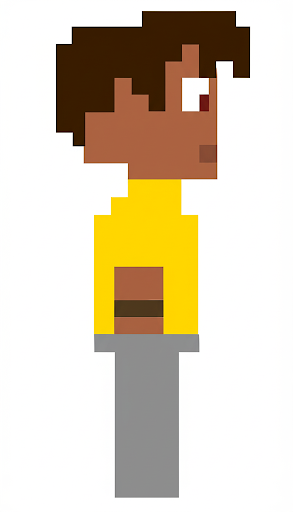
\includegraphics[width=0.3\linewidth]{figs/geminiPro/chat6/tela2_res4.png}
    \legend{\small Fonte: Elaborada pela autora, utilizando a ferramenta Gemini Pro.}
\end{figure}

Como esperado, os resultados demonstraram inconsistência com o estilo, como se estivessem usando como base apenas as características do personagem e ignorando as imagens de referência, o que pode ser visto na Figura \ref{fig:GeminiProSpriteSheetInconsistente}. Isso contribui para a hipótese anterior, sobre o modelo de chat estar enviando apenas o prompt textual para o Imagen 4 por causa do envio das imagens numa mensagem diferente. Para consolidar essa teoria, mais testes foram realizados utilizando um prompt idêntico com a imagem anexada na mesma mensagem. Porém, antes de abordar esses novos experimentos, é importante ressaltar outras características presentes em todas as figuras geradas. A IA foi capaz de fazer 16 quadros, porém — como aconteceu durante a análise de outras ferramentas — o mesmo sprite era repetido com mudanças não significativas, sem formar o movimento de caminhada. 


\begin{figure}[htbp]
    \centering
    \caption{\small Sprite sheet inconsistente gerado no Gemini Pro}
    \label{fig:GeminiProSpriteSheetInconsistente}
    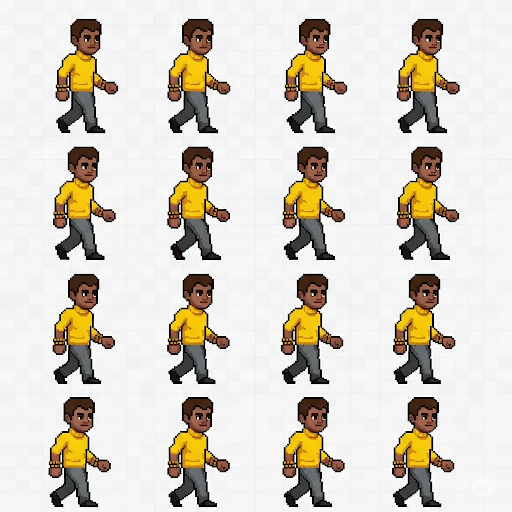
\includegraphics[width=0.5\linewidth]{figs/geminiPro/chat8/tela1_res5.PNG}
    \legend{\small Fonte: Elaborada pela autora, utilizando a ferramenta Gemini Pro.}
\end{figure}

Continuando os testes, foi anexada a melhor imagem do personagem em side view gerada (que naquele momento era a Figura \ref{fig:GeminiProSideMelhor}) e repetido o mesmo prompt de antes. De maneira inesperada, os resultados apresentaram consistência variável com o estilo, como pode ser visto na Figura \ref{fig:GeminiProSpriteSheetConsistenciaVariavel}. Além disso, o número de quadros gerados foi diferente do valor instruído, possuindo diversos frames repetidos, porém eventualmente mudando a pose para avançar o movimento (o que não ocorreu na geração anterior). Todos os resultados podem ser consultados na Figura \ref{fig:geminiProSheet2} no Apêndice \ref{ap.telasIA}.

\begin{figure}[htbp]
    \centering
    \caption{\small Sprite sheet parcialmente inconsistente gerado no Gemini Pro}
    \label{fig:GeminiProSpriteSheetConsistenciaVariavel}
    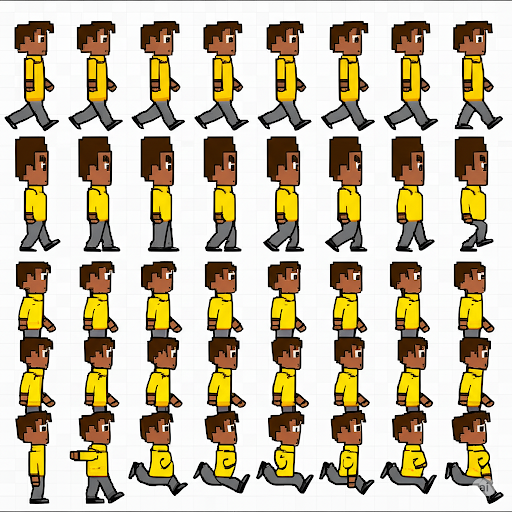
\includegraphics[width=0.5\linewidth]{figs/geminiPro/chat8/tela2_res1.PNG}
    \legend{\small Fonte: Elaborada pela autora, utilizando a ferramenta Gemini Pro.}
\end{figure}

Analisando a fundo, foi levantada a teoria de que os resultados podem ter sido influenciados pelo contexto já existente da ferramenta, pois ambas as baterias de testes foram realizadas no mesmo chat. Isso explicaria o motivo de algumas imagens geradas manterem a consistência com a figura anexada, enquanto outras apresentavam a mesma inconsistência do experimento anterior. Para eliminar essa interferência, foi criado um novo chat, onde replicou-se de maneira exata o teste inicial (utilizando as Figuras \ref{fig:geminiProPablo} e \ref{fig:GeminiProSpriteSheetSide}), exceto pelo fato de que os textos (descrição, contexto e prompt) foram unidos em uma só mensagem. 

Os resultados apresentaram uma consistência maior do que os testes anteriores, mantendo características específicas das referências, porém perdendo o estilo de pixel art e com diversas deformações no sprite, como pode ser visto na Figura \ref{fig:GeminiProSpriteSheetMelhor1}. O erro de frames sem mudanças significativas diminuiu, porém foram gerados mais do que 16 quadros e algumas posições apareceram de forma imprecisa . Em alguns casos, o personagem era desconstruído ou parecia fazer ações diferentes do que apenas andar, como pode ser observado na Figura \ref{fig:GeminiProSpriteSheetDesconstruido}. Em geral, apesar de mostrarem uma semelhança maior com o estilo da imagem de referência, os resultados foram menos precisos, com mais deformações e menos satisfatórios quando considerada apenas a descrição textual do personagem. A interação completa pode ser consultada na Figura \ref{fig:geminiPro3} no Apêndice \ref{ap.telasIA}.

\begin{figure}[htbp]
    \centering
    \caption{\small Melhor sprite sheet do personagem andando utilizando várias imagens de referência na mesma mensagem do prompt gerado no Gemini Pro}
    \label{fig:GeminiProSpriteSheetMelhor1}
    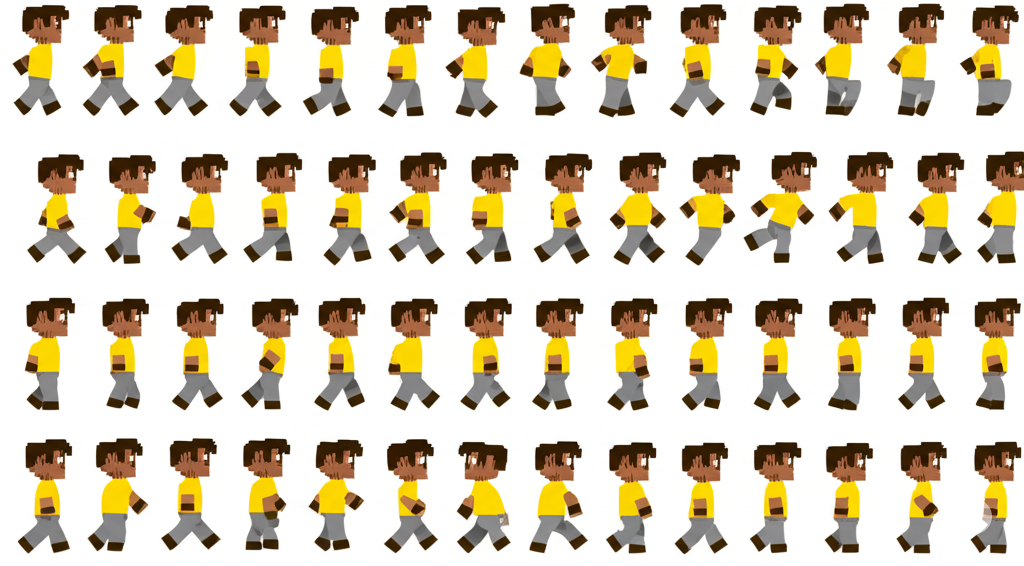
\includegraphics[width=0.8\linewidth]{figs/geminiPro/chat9/1res1.PNG}
    \legend{\small Fonte: Elaborada pela autora, utilizando a ferramenta Gemini Pro.}
\end{figure}

\begin{figure}[htbp]
    \centering
    \caption{\small Sprite sheet com o personagem mantendo diferentes partes do desenho gerado no Gemini Pro}
    \label{fig:GeminiProSpriteSheetDesconstruido}
    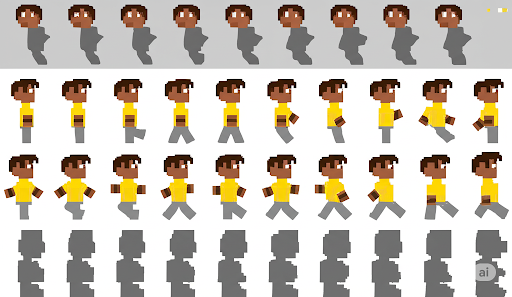
\includegraphics[width=0.6\linewidth]{figs/geminiPro/chat9/1res5.PNG}
    \legend{\small Fonte: Elaborada pela autora, utilizando a ferramenta Gemini Pro.}
\end{figure}

Nos testes seguintes, voltou-se a anexar apenas a melhor imagem gerada em side view até aquele momento (Figura \ref{fig:GeminiProSideMelhor}). 

Quando era usado o mesmo chat, geraram-se sprites mais parecidos com o de referência e com levemente menos deformações, porém ainda mantendo as demais características comentadas anteriormente (Figura \ref{fig:geminiPro4} no Apêndice \ref{ap.telasIA}). 

Entretanto, ao se utilizar um novo chat, a consistência do personagem e do estilo aumentou de forma satisfatória na maioria das figuras geradas, com um número menor de deformações em comparação com os outros resultados, como pode ser visto na Figura \ref{fig:GeminiProSpriteSheetMelhor}. De maneira inesperada, essa estratégia gerou, em certos momentos, sequências de imagens com os sprites em vez de uma imagem com o sprite sheet, além de apresentar uma maior repetição de quadros sem mudança significativa.  Os resultados completos podem ser verificados na Figura \ref{fig:geminiPro5} no Apêndice \ref{ap.telasIA}.

\begin{figure}[htbp]
    \centering
    \caption{\small Melhor sprite sheet gerado no Gemini Pro}
    \label{fig:GeminiProSpriteSheetMelhor}
    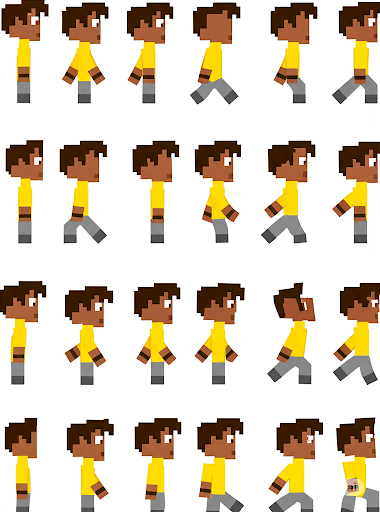
\includegraphics[width=0.5\linewidth]{figs/geminiPro/chat10/tela1_res3.PNG}
    \legend{\small Fonte: Elaborada pela autora, utilizando a ferramenta Gemini Pro.}
\end{figure}

\begin{quadro}[htbp]
    \centering
    \caption{\small Resumo dos experimentos de geração do sprite sheet no Gemini Pro}
    \label{quadro:GeminiProSpriteSheet}
    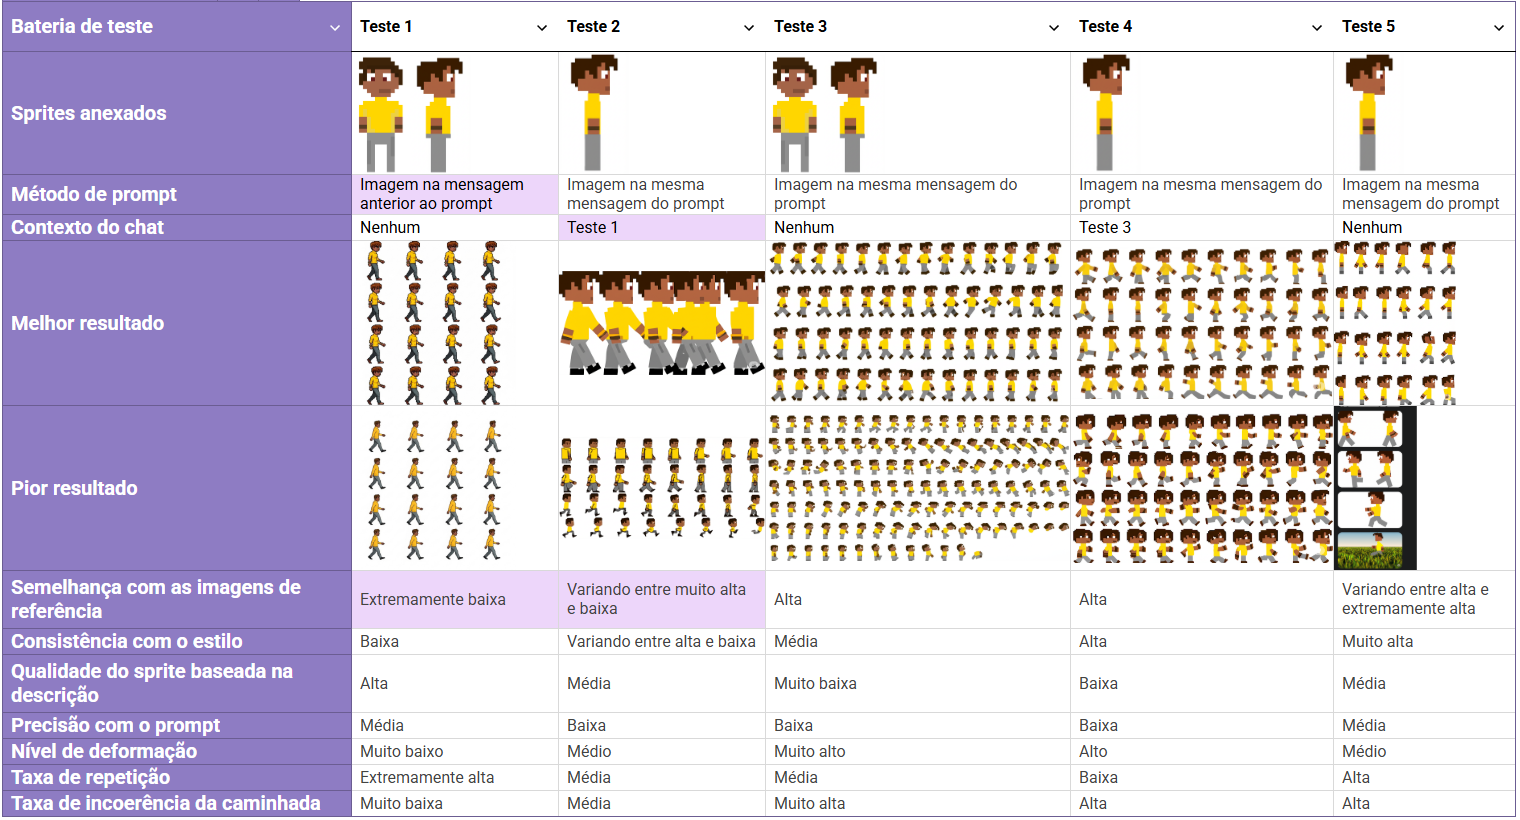
\includegraphics[width=1\linewidth]{figs/geminiPro/tabela_geracao_sprite_sheet.PNG}
    \legend{\small Fonte: Elaborada pela autora.}
\end{quadro}


Analisando e comparando todos os resultados, compilados no Quadro \ref{quadro:GeminiProSpriteSheet}, é consolidada a hipótese sobre a importância de anexar as imagens de referência na mesma mensagem do prompt. A provável causa desse comportamento é que o modelo de chat não retém o conteúdo visual de mensagens anteriores que não tiverem relação com uma geração da imagem, dessa forma não podendo enviar a figura ao formular a instrução para o Imagen 4.

Os experimentos também revelaram que a ferramenta Gemini Pro apresenta dificuldades em gerar sequências de imagens com pequenas variações. A IA tende a repetir quadros e poses, introduzir deformações ou perder a precisão da progressão do movimento ao tentar criar os múltiplos sprites de uma animação. Conclui-se que, embora excelente para a criação de sprites específicos, o Gemini Pro não se mostrou capaz de formar o sprite sheet de uma animação, falhando em compreender o contexto temporal de um ciclo de caminhada.

